%%%%%%%%%%%%%%%%%%%%%%%%%%%%%%%%%%%%%%%%%%%%%%%%%%%%%%%%%%%%%%%%%%%%
% This is a thesis template for Gebze Technical University.
%
% Please only edit the areas proceeded by a comment starting with %%
% otherwise the template may be broken.
%
% This file is only to be used for editing the general fields
% and inputting the body of the thesis in the designated areas.
% Please write the body of the thesis in separate files, and input
% them as shown in the comment preceding the area.
%
% Created in Aug 2021 by Usama Derbashi.
%%%%%%%%%%%%%%%%%%%%%%%%%%%%%%%%%%%%%%%%%%%%%%%%%%%%%%%%%%%%%%%%%%%%
\documentclass[12pt]{report}


% Language and typeset setting
\usepackage[english]{babel}
\usepackage[a4paper,top=25mm,bottom=25mm,left=40mm,right=25mm]{geometry}
\usepackage[onehalfspacing]{setspace}
\usepackage{algorithm, algpseudocode}
\usepackage{indentfirst}
\setlength{\parindent}{1cm}
\setlength{\abovecaptionskip}{12pt plus 0pt minus 0pt}
\setlength{\belowcaptionskip}{12pt plus 0pt minus 0pt}
\setlength{\textfloatsep}{18.0pt plus 0.0pt minus 0.0pt}
\setlength{\floatsep}{18.0pt plus 0.0pt minus 0.0pt}
\setlength{\intextsep}{18.0pt plus 0.0pt minus 0.0pt}
\setlength{\skip\footins}{18.0pt plus 0.0pt minus 0.0pt}

% Core packages and settings
\usepackage[colorlinks=false]{hyperref}
\usepackage{amsmath}

\usepackage{titlesec} %setting the titles of chapters and sections
\setcounter{secnumdepth}{4}
\setcounter{tocdepth}{4}
\titleformat{\chapter}[hang]{\normalfont\bfseries\MakeUppercase}{}{0pt}{\LARGE\thechapter. }
\titleformat{\section}[hang]{\normalfont\bfseries}{}{0pt}{\Large\thesection. }
\titleformat{\subsection}[hang]{\normalfont\bfseries}{}{0pt}{\large\thesubsection. }
\titleformat{\subsubsection}[hang]{\normalfont\bfseries}{}{0pt}{\large\thesubsubsection. }
\titlespacing*{\chapter}{0pt}{0pt}{18pt}
\titlespacing*{\section}{0pt}{18pt}{18pt}
\titlespacing*{\subsection}{0pt}{18pt}{18pt}
\titlespacing*{\subsubsection}{0pt}{18pt}{18pt}

\usepackage{graphicx}
\graphicspath{{./Imgs/}} %pointing the directory of images

\usepackage{fancyhdr} % setting footers
\usepackage{etoolbox} 
\renewcommand{\headrulewidth}{0pt}
\patchcmd{\chapter}{\thispagestyle{plain}}{\thispagestyle{fancy}}{}{}
\pagestyle{fancy}
\fancyhf{}
\fancyfoot[C]{\fontsize{11pt}{11pt}\thepage}

\usepackage[style=ieee]{biblatex}
\addbibresource{refs.bib}
\usepackage{csquotes}% Needed for babel(in biblatex)

\usepackage[bottom, perpage]{footmisc}%% amkes footnotes at the bottom

\usepackage{GTUThesis}


% Additional packages if needed
%% For the sake of not messing the template add them here

\usepackage{xcolor}
\definecolor{light-blue}{HTML}{6b85dd}
\definecolor{dark-blue}{HTML}{4266d5}
\definecolor{light-red}{HTML}{d66661}
\definecolor{dark-red}{HTML}{c93d39}
\definecolor{light-green}{HTML}{6bab5b}
\definecolor{dark-green}{HTML}{3b972e}
\definecolor{light-purple}{HTML}{aa7dc0}
\definecolor{dark-purple}{HTML}{945bb0}
\usepackage{listings, minted}

\usepackage{multicol}
\usepackage{changepage}
\usepackage[export]{adjustbox}
\usepackage{lipsum}


% Important information
%% Make sure to enter all the info below
\title{Polynomiography}
\author{İSMAİL TAPAN}
\faculty{Faculty of Engineering}
\department{Computer Engineering Department}
\supervisor{Dr. Tülay Ayyıldız Akoğlu}
\theyear{2023}


\begin{document}

%Front Matter
\pagenumbering{roman} %start with roman numbering 
\projecttitlepageenglish
\maketitle
\setcounter{page}{3} %the first two title pages are not counted so this is a buffer
\begin{outertitles} % makes titles centred

%% below enter as follows 
%% {DATE_OF_DEMO}{JURY}
%% Note that JURY should be comma separated
\makejury{19/01/2023}{Prof. Dr. Didem GÖZÜPEK}
\chapter*{Abstract}
\addcontentsline{toc}{chapter}{Abstract}

Polynomiography is a a visual art form that involves visualization of complex polynomials.

...

In this work we will explore new methods to generate  artistic images/image sequences from polynomials. We will create a Python library to help people use and improve these methods for generating artistic images from polynomials. Our goal is to encourage more research and experimentation in this area by sharing these methods as open-source software.

\vfill

\textbf{Keywords:} Polynomial, Polynomiography, Digital Art
\clearpage
% \chapter*{List of Symbols and Abbreviations}
\addcontentsline{toc}{chapter}{List of Symbols and Abbreviations}

\begin{tabular}{lcl}
    \textbf{Symbol or}&&\\
    \textbf{Abbreviation} &:& \textbf{Explanation}\\
    
    %% Edit below in the format
    %% XYZ &:& EXPLANATION\\
    %% where XYZ is the acronym or symbol
    %% and EXPLANATION is the explanation of it
    %% make sure not to forget &:& between them, and \\ at the end of EXPLANATION

    %$\mu$ &:& Small mu\\
    
    %% Until here
\end{tabular}

\clearpage

\tableofcontents
\addcontentsline{toc}{chapter}{Contents}
\clearpage

\listoffigures
\addcontentsline{toc}{chapter}{List of Figures}
\clearpage

\listoftables
\addcontentsline{toc}{chapter}{List of Tables}
\clearpage

\end{outertitles}
\fancyhf{}%reset footer
\fancyfoot[R]{\fontsize{11pt}{11pt}\thepage}%page numbers in the corner
\addtocontents{toc}{\protect\vspace{18pt}}
\pagenumbering{arabic}%turn to arabic numbers

% Mainmatter

%% Only input files, don't write here
%% \input{./Body/Mainmatter/FILE}
\chapter{Introduction}

\section{Polynomials}
// TODO: extend this to polynomial rings

A polynomial is a mathematical expression of the form:

\begin{center}
$a_nz^n +a_{n-1}z^{n-1} + \cdots + a_1z+a_0$
\end{center}

where $a_n$, $a_{n-1}$, $\dots$, $a_0$ are coefficients, $n$ is the degree, $a_n$ is nonzero, and $z$ is a variable.

The degree of a polynomial is the highest power of the variable $z$ in the expression. For example, the polynomial $3z^2 + 2z - 1$ has degree 2, while the polynomial $4z^3 + 7z^2 - 5z + 1$ has degree 3.

A polynomial equation is an equation of the form:

\begin{center}
$a_nz^n +a_{n-1}z^{n-1} + \cdots + a_1z+a_0 = 0$
\end{center}

A solution, or root, of a polynomial is any specific value of $z$ that would satisfy the polynomial equation.

\subsection{Polynomial Rings over Finite Fields}
A polynomial ring over a finite field is a set of polynomials with coefficients taken from a finite field. Given a finite field $F_q$ with $q$ elements, the polynomial ring over $F_q$ is denoted by $F_q[x]$ and the elements of $F_q[x]$ are polynomials of the form:

\begin{center}
$f(x) = a_0 + a_1x + a_2x^2 + \cdots + a_nx^n$
\end{center}

where $a_0, a_1, \dots, a_n \in F_q$ and $n$ is a non-negative integer.

(e.g.) All degree 3 polynomials of $F_q[x]$ where $F_q = {0, 1}$:
\begin{multicols}{4}
\begin{itemize}
    \item $x^3$
    \item $x^3 + 1$
    \item $x^3 + x$
    \item $x^3 + x + 1$
    \item $x^3 + x^2$
    \item $x^3 + x^2 + 1$
    \item $x^3 + x^2 + x$
    \item $x^3 + x^2 + x + 1$
\end{itemize}
\end{multicols}

\section{Root finding algorithms}

In mathematics and computing, a root algorithm is an algorithm for finding roots of continuous polynomial functions. Most of the root finding algorithms are iteration based, they require one or more initial values and try to converge to the a root of the function in each iteration. These methods don't find an exact solution but an approximation to a root.

\lstset{
  basicstyle=\footnotesize,
  mathescape
}

\subsection{Iterative methods}
\subsubsection{Householder's methods (Derivative Based Methods)}
    It's an iterative method that uses this generic formula to converge to a root:
    \[x_{n+1}=x_{n}+d{\frac {(1/f)^{(d-1)}(x_{n})}{(1/f)^{(d)}(x_{n})}}\]

    where $f^{(n)}$ denotes the $(n)$th derivative of $f$.

    The methods that uses first two order of this formula have special names, Newton's Method and Halley's method respectively.
    
\paragraph{Newton's Method} 
    $\newline$
    If you plug 1 as d in the previous formula, you get the following formula:
    \[x_{n+1}=x_{n}+{\frac {(1/f)(x_{n})}{(1/f)^{(1)}(x_{n})}}\]
    \[x_{n+1}=x_{n}+{\frac {\frac{1}{f(x_{n})}}{-\frac{f'(x_{n})}{f^2(x_{n})}}}\]
    \[x_{n+1}=x_{n}+{\frac {1}{f(x_{n})}(-\frac{f^2(x_{n})}{f'(x_{n})})}\]    
    \[x_{n+1} = x_n - \frac{f(x_n)}{f'(x_n)}\]
    
So the algorithm will be as follow:
\begin{lstlisting}
        1 - Start with some $x$
        2 - Iterate the following formula until the difference 
        between $x_n$ and $x_{n+1}$ is less then some $\epsilon$
                $x_{n+1} = x_n - \frac{f(x_n)}{f'(x_n)}$
        3 - Return the approximated value [and iteration count]
\end{lstlisting}
\paragraph{Halley's Method}
    $\newline$
    If you plug 2 as d in the previous formula, you get the following formula:
    \[x_{n+1}=x_{n}+{\frac {(1/f)^{(1)}(x_{n})}{(1/f)^{(2)}(x_{n})}}\]
    \[x_{n+1}=x_{n}+{\frac{-\frac{f'(x_{n})}{f^2(x_{n})}}{\frac{f''(x_{n})}{f^2(x_{n})} - 2\frac{f'(x_{n})f'(x_{n})}{f^3(x_{n})}}}\]
    \[x_{n+1}=x_{n}+{(-\frac{f'(x_{n})}{f^2(x_{n})}) (\frac{f''(x_{n})}{f^2(x_{n})} - 2\frac{f'(x_{n})f'(x_{n})}{f^3(x_{n})})^{-1} }\] 
    \[x_{n+1}=x_{n}+{(-\frac{f'(x_{n})}{f^2(x_{n})}) (\frac{f(x_{n})f''(x_{n}) - 2f'(x_{n})f'(x_{n})}{f^3(x_{n})})^{-1} }\]
    \[x_{n+1}=x_{n}+{(-\frac{f'(x_{n})}{f^2(x_{n})}) (\frac{f^3(x_{n})}{f(x_{n})f''(x_{n}) - 2f'(x_{n})f'(x_{n})}) }\]
    \[x_{n+1} = x_n -\frac{f(x_{n})f'(x_{n})}{2f'(x_{n})f'(x_{n}) - f(x_{n})f''(x_{n})}\]

So the algorithm will be as follow:
\begin{lstlisting}
    1 - Start with some $x$
    2 - Iterate the following formula until the difference 
    between $x_n$ and $x_{n+1}$ is less then some $\epsilon$
            $x_{n+1} = x_n -\frac{f(x_{n})f'(x_{n})}{2f'(x_{n})f'(x_{n}) - f(x_{n})f''(x_{n})}$
    3 - Return the approximated value [and iteration count]
\end{lstlisting}


\paragraph{Others}
    $\newline$
This method can be implemented for higher orders too. The only thing that will change is the formula that computes the next iteration in the algorithm.

A general algorithm can be written as:
\begin{lstlisting}
    1 - Start with some $x$
    2 - Iterate the following formula until the difference 
    between $x_n$ and $x_{n+1}$ is less then some $\epsilon$
            $x_{n+1} =$ //$x_n$ plugged into derived formula
    3 - Return the approximated value [and iteration count]
\end{lstlisting}

\newpage
\subsubsection{Steffensen's Method}
// TODO: maybe explain how it is obtained or cite

In this method the next iteration is computed with the following formula:
\[x_{n+1} = x_n -\frac{f(x_{n})}{\frac{f(x_n + f(x_n))}{f(x_n)} - 1}\]


So the algorithm will be as follow:
\begin{lstlisting}
    1 - Start with some $x$
    2 - Iterate the following formula until the difference 
    between $x_n$ and $x_{n+1}$ is less then some $\epsilon$
            $x_{n+1} = x_n -\frac{f(x_{n})}{\frac{f(x_n + f(x_n))}{f(x_n)} - 1}$
    3 - Return the approximated value [and iteration count]
\end{lstlisting}


\subsubsection{Secant Method}
    // TODO: implement

\subsubsection{Inverse Interpolation}
    // TODO: implement

\subsection{Bracketing methods}
    // note sure if it's possible to implement bracketing methods for polynomiography since we will need one input that gives positive and one input that gives negative result to start
\subsubsection{Bisection Method}
    // TODO: implement
    
\subsubsection{False Position (Regula Falsi)}
    // TODO: implement
    
\subsection{Combinations of methods}
\subsubsection{Brent's Method}
    Combination of bisection method, the secant method and inverse quadratic interpolation.
    
    // note sure if it's possible to implement bracketing methods for polynomiography since we will need one input that gives positive and one input that gives negative result to start
    
    // TODO: implement



\chapter{Implementation}

\section{Project Design}
// Update these pictures
\begin{figure}[!htbp]
    \label{fig:project-design}
    Use Case 1
    \begin{center}
    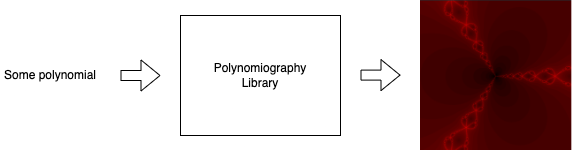
\includegraphics[width=0.8\textwidth]{Imgs/fig2.png}    
    \end{center}
    Use Case 2
    \begin{center}
    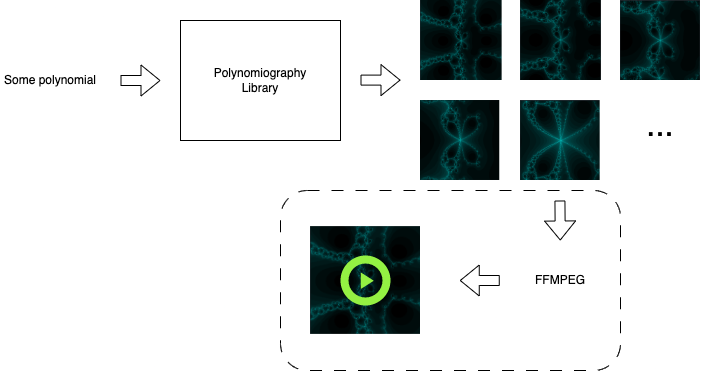
\includegraphics[width=0.8\textwidth]{Imgs/fig3.png}  
    \end{center}
    Use Case 3
    \begin{center}
    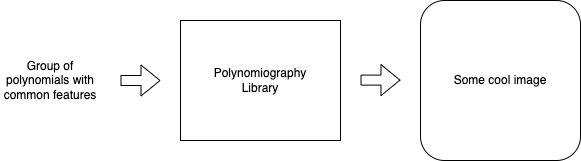
\includegraphics[width=0.8\textwidth]{Imgs/fig6.png}
    \caption{High Level Project Design}
    \end{center}
\end{figure}

\section{Implementation Details}

\subsection{Canvas $\iff$ Complex Plane}

\begin{figure}[!htbp]
    \centering
    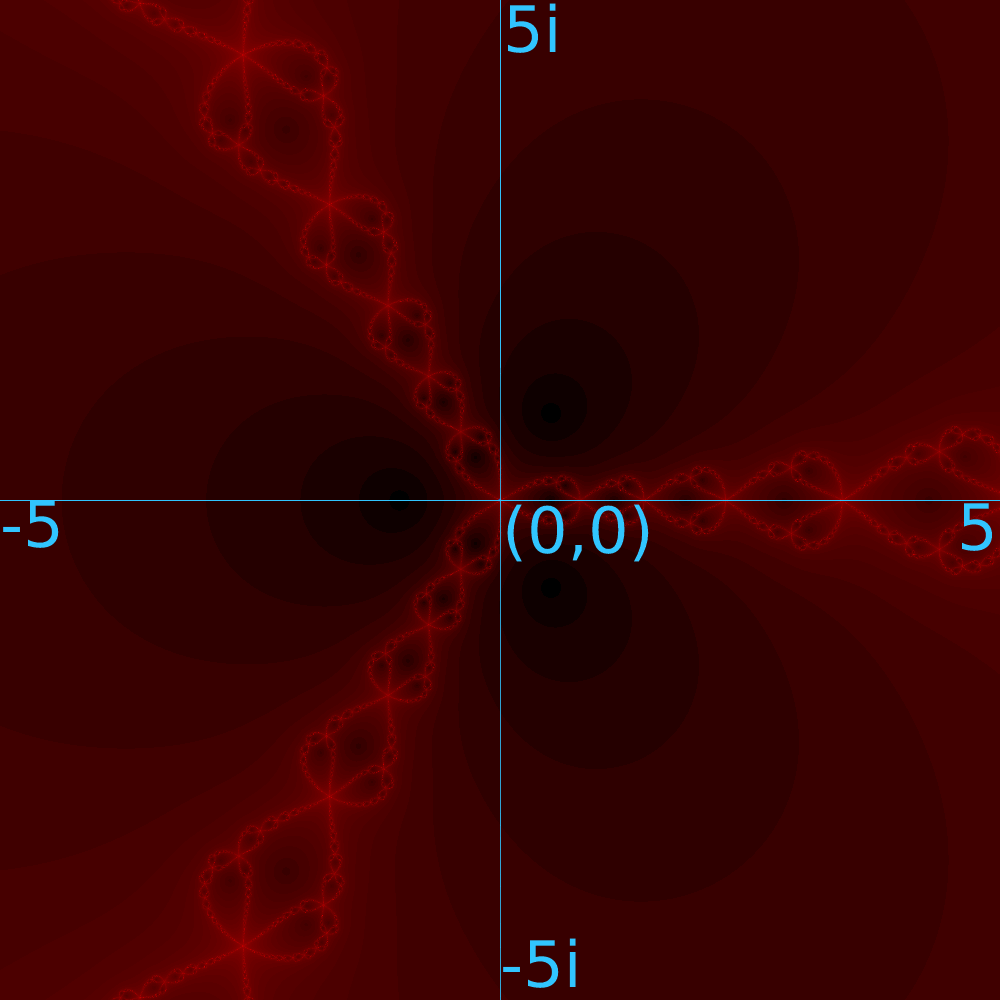
\includegraphics[width=0.6\textwidth]{Imgs/fig4.png}
    \caption{Complex plane on canvas}
    \label{fig:canvas-complex-plane}
\end{figure}

\subsection{Visualization of Iterative Root Finding Methods}

// Elaborate\\
-   For each pixel find the corresponding complex number\\
-   Start the iterative method with the corresponding number\\
-   Get the total iteration count until it converges\\
-   Assign a color to this pixel with respect to iteration count\\

\subsection{Visualization of Roots of Polynomial Rings Over Finite Fields}

// Elaborate\\
-   Compute the roots for each polynomial in finite field \\
-   Iterate over each root, find the corresponding pixel from the complex number\\
-   Increase the color on that pixel\\

\section{Usage}

For detailed usage see \hyperref[Appendix 1]{API Documentation}

\chapter{Results}

\chapter{Conclusions}




% DON'T INPUT FILES AFTER HERE
\begin{outertitles}
\clearpage
\setlength{\emergencystretch}{1em}
\printbibliography
\addtocontents{toc}{\protect\vspace{18pt}}
\addcontentsline{toc}{chapter}{Bibliography}
%% If you don't want a CV or appendices add a % at the beginning of the relevant line
% \chapter*{CV}
\addcontentsline{toc}{chapter}{CV}

%% Edit below this line
XXX.



%% Until here
\clearpage
\chapter*{Appendices}
\addcontentsline{toc}{chapter}{Appendices}

\section*{Appendix 1: API Documentation}

// Documentation of the Polynomiogra\textbf{py} library

\label{Appendix 1}
\end{outertitles}
\end{document}